% ============================ PHASE 3 ==================================
\newpage
\phase{Phase three \textbullet\ The machine}{Choosing the electrolyser stack}{Five ways to split water, judged on market availability, cost, supply chain, risk and the value each rupee buys.}

\subsection{What a green hydrogen plant actually is}

The electrolyser gets the headlines, but it is only the heart of a much larger body. A green-ammonia plant is really three plants bolted together: a power plant, a hydrogen plant and a chemical plant.

\begin{figure}[H]
\centering
\begin{tikzpicture}[
  blk/.style={rounded corners=2pt,draw=#1,line width=0.8pt,fill=paper,align=center,font=\footnotesize,minimum height=11mm,text width=20mm,inner sep=2pt},
  hot/.style={rounded corners=2pt,fill=ink,text=paper,align=center,font=\footnotesize\bfseries,minimum height=13mm,text width=22mm},
  ar/.style={-{Stealth[length=2.2mm]},line width=0.8pt,color=ink2},
  grp/.style={rounded corners=4pt,draw=rule,line width=0.6pt,dashed,inner sep=2.2mm},
  gl/.style={font=\eyebrowfont\fontsize{6.2}{7}\selectfont,text=brass,anchor=north west}]
\node[blk=sochre] (sol) {Solar + wind\\ farms};
\node[blk=sochre,below=4mm of sol] (bat) {Battery\\ (optional)};
\node[blk=ink2,right=6mm of sol,yshift=-7.5mm] (rec) {Transformer +\\ rectifier (AC$\rightarrow$DC)};
\node[hot,right=17mm of rec] (ely) {ELECTROLYSER\\ STACKS};
\node[blk=sblue,below=7mm of ely,xshift=-12.5mm] (wat) {Water treatment\\ (RO / desalination)};
\node[blk=sviolet,below=7mm of ely,xshift=12.5mm] (o2) {Oxygen\\ (vent or sell)};
\node[blk=ink2,right=17mm of ely,yshift=7.5mm] (cmp) {Compressor +\\ hydrogen buffer};
\node[blk=ink2,below=4mm of cmp] (asu) {Air separation\\ (nitrogen)};
\node[blk=sgreen,right=6mm of cmp,yshift=-7.5mm] (hb) {Haber–Bosch\\ ammonia loop};
\node[blk=sgreen,below=7mm of hb] (tank) {Ammonia tank\\ $\rightarrow$ customer};
\draw[ar] (sol.east) -- ++(2mm,0) |- ([yshift=2mm]rec.west); \draw[ar] (bat.east) -- ++(2mm,0) |- ([yshift=-2mm]rec.west);
\draw[ar] (rec) -- (ely);
\draw[ar] (wat.north) -- (wat.north |- ely.south);
\draw[ar] (o2.north |- ely.south) -- (o2.north);
\draw[ar] (ely.east) -- ++(4mm,0) |- (cmp.west);
\draw[ar] (cmp.east) -- ++(2mm,0) |- ([yshift=2mm]hb.west);
\draw[ar] (asu.east) -- ++(2mm,0) |- ([yshift=-2mm]hb.west);
\draw[ar] (hb) -- (tank);
\begin{scope}[on background layer]
\node[grp,fit=(sol)(bat)(rec)] (g1) {}; \node[gl] at (g1.south west) {POWER PLANT};
\node[grp,fit=(wat)(ely)(o2)] (g2) {}; \node[gl] at (g2.south west) {HYDROGEN PLANT};
\node[grp,fit=(cmp)(asu)(hb)(tank)] (g3) {}; \node[gl] at (g3.south west) {CHEMICAL PLANT};
\end{scope}
\end{tikzpicture}
\caption{The parts of a green-ammonia plant. Everything except the dark box is ``balance of plant'', and it is where cost overruns usually hide.}
\end{figure}

\begin{plainwords}
The price tag on the electrolyser is not the price of the plant. The IEA finds that a Chinese-made electrolyser installed in China costs \usd{}500–1,100 per kW all-in, while systems made outside China cost \usd{}1,900–2,500 per kW installed. Once a Chinese unit is shipped abroad, engineering and contingency costs ``narrow the gap sharply'' \cite{argus2026}. So when someone quotes a \usd{}300 stack, ask what the transformer, compressor, water plant, civil works and contingency add. \confH
\end{plainwords}

\subsection{The five stacks, in plain words}

There are four basic ways to split water with electricity, and one sensible blend of two of them. I treat each as a ``stack'' we could build the project on.

\begin{table}[H]\centering\tablefont
\caption{The five candidate stacks. Efficiency, life and materials are IRENA's 2020 state of the art \cite{irena2020}; flexibility from \cite{ammoniaenergy2023}; 2025–26 status from the sources cited.}
\begin{tabularx}{\textwidth}{@{}p{19mm} L L L L@{}}
\toprule
& \thead{How it works} & \thead{Efficiency \& life} & \thead{Flexibility \& materials} & \thead{Where it stands, 2026}\\ \midrule
\textbf{Alkaline (pressurised)} & Nickel-coated steel electrodes in a caustic potash bath, 70–90\,°C & 50–78 kWh/kg; stack about 60,000 h & Pressurised units turn down only to about 40\% load, atmospheric to 15\%; nickel and steel, no precious metals & The workhorse. Most Chinese makers build it \cite{hfn2025}; a 1 MW unit fell from about \usd{}800 to \usd{}400/kW in three years \cite{hfn2025}. \confH\\
\textbf{PEM} & A thin acid polymer membrane; iridium oxide and platinum catalysts, 50–80\,°C & 50–83 kWh/kg; 50,000–80,000 h & Follows solar and wind closely; needs very pure water; relies on iridium & Commercial, pricier. Iridium is the long-run choke point (Section~\ref{sec:supply}). \confH\\
\textbf{Hybrid ALK + PEM} & Alkaline for the steady base, a PEM slice for the swings & Weighted mix of the two & Captures more renewable hours than alkaline alone & An engineering choice, not a product. Needs two OEMs and good controls. \confM\\
\textbf{AEM} & A membrane like PEM, but alkaline chemistry with cheap nickel catalysts, 40–60\,°C & 57–69 kWh/kg; durability was above 5,000 h in 2020 & Promises PEM-like flexibility without precious metals & First 5 MW system delivered in April 2026; an Indian 250–300 MW factory announced via a US licence \cite{enki2026}. Durability is the open question. \confL\\
\textbf{SOEC} & Ceramic cells at 700–850\,°C splitting steam & 45–55 kWh/kg (plus heat); under 20,000 h & Must run hot and steady; ceramics and perovskites & Leading maker Topsoe will ``hibernate'' its factory until demand is robust and dropped a planned US plant (June 2026) \cite{h2central2026}. \confH\\
\bottomrule
\end{tabularx}
\end{table}

\subsection{Market availability: a buyer's market for proven kit}

The electrolyser industry has built far more factories than the world is buying from. Global manufacturing capacity reached almost 58 GW a year by the end of 2025, about 60\% of it in China, 20\% in Europe and 10\% in the US. Actual output was under 5 GW, a utilisation of roughly 9\%, and the IEA says the sector is ``entering a consolidation phase''; Cummins, for one, has stopped selling electrolysers once existing orders are filled \cite{argus2026}. China also hosts about 65\% of the electrolyser capacity that is installed or at final investment decision worldwide \cite{ieanews2025}. India has awarded 3,000 MW a year of electrolyser manufacturing capacity to 15 firms under its incentive scheme \cite{rw2025}. \confH

\begin{finding}[What the glut means for us]
For alkaline and PEM, we are the customer in a buyer's market. We can demand long warranties, performance guarantees and service agreements, because suppliers need the orders. The flip side is \emph{supplier survival risk}: an OEM that goes bust in year six cannot honour a 10-year stack guarantee. For AEM and SOEC the market is the opposite: thin, early and unproven. \confM
\end{finding}

\subsection{Cost of production: what a kilogram really costs}\label{sec:cost}

I built a small model to put all five stacks on the same footing. It asks one question: \emph{over 25 years, what does each kilogram of hydrogen cost once every rupee of capital, maintenance, stack replacement and electricity is counted?} Economists call this the levelised cost of hydrogen (LCOH):
\[
\text{LCOH} = \frac{\overbrace{\text{Capex}\times\text{CRF}}^{\text{paying back the plant}} + \overbrace{\text{O\&M}}^{\text{upkeep}} + \overbrace{\text{Stack replacement}}^{\text{wear and tear}}}{\text{kg of hydrogen made per year}} \;+\; \underbrace{\text{Electricity price}\times\text{kWh per kg}}_{\text{the power bill}} \;+\; \text{water}
\]
The capital recovery factor (CRF) turns a one-time cost into an equal yearly payment at the cost of capital, exactly like an EMI on a home loan. The full input table is in Annex B. The four inputs that matter most are:

\begin{itemize}
\item \textbf{Electricity:} \usd{}32–48 per MWh, base \usd{}38. The low end is the ₹2.86/kWh discovered for solar plus four-hour storage in October 2025 \cite{sqsolar2025}. Round-the-clock firm power costs ₹5.25/kWh (about \usd{}58) \cite{pvmfdre2026}, which I use only for SOEC because it cannot follow the sun. \confM
\item \textbf{Cost of capital:} 8.5–12.5\%, base 10\%. This is my assumption; Gemini's brief estimated 9.5–11.5\% \cite{gemini2026}. \confL
\item \textbf{Renewable hours:} an oversized solar-plus-wind farm can feed the stack 55–68\% of the hours in a year. Alkaline captures 92\% of those hours because of its high minimum load; PEM captures 99\%. \confL
\item \textbf{Installed cost:} alkaline \usd{}800–1,600 per kW, PEM \usd{}1,300–2,400, AEM \usd{}1,000–3,000, SOEC \usd{}2,800–5,600, all anchored on the IEA and IRENA ranges \cite{argus2026,irena2020,h2techcapex2022}. \confM
\end{itemize}

\begin{figure}[H]
\centering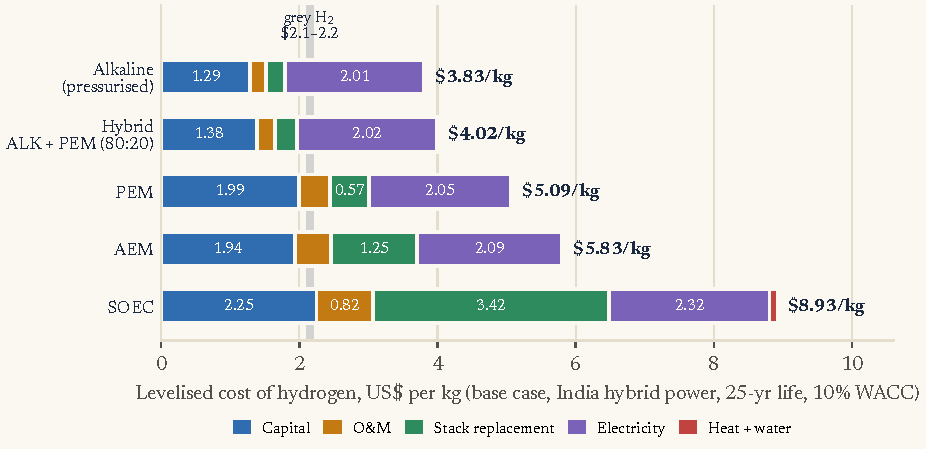
\includegraphics[width=\textwidth]{figures/lcoh_stack.pdf}
\caption{Base-case cost of a kilogram of green hydrogen, split by where the money goes. Grey hydrogen in India: \cite{jmkiocl2025,tribune2025}.}
\end{figure}

The base case puts \textbf{alkaline at \usd{}3.83/kg}, the hybrid \usd{}0.19 dearer, PEM \usd{}1.26 dearer, AEM \usd{}2.00 dearer and SOEC more than double. That alkaline figure sits inside the \usd{}3.5–4/kg that market analysts quote for Indian green hydrogen today \cite{tribune2025}, which is my main check that the model is calibrated. \confM

A single number hides the risk, so I ran each stack through 100,000 simulated futures, drawing every uncertain input from its low–likely–high range (Figure~\ref{fig:mc}).

\begin{figure}[H]
\centering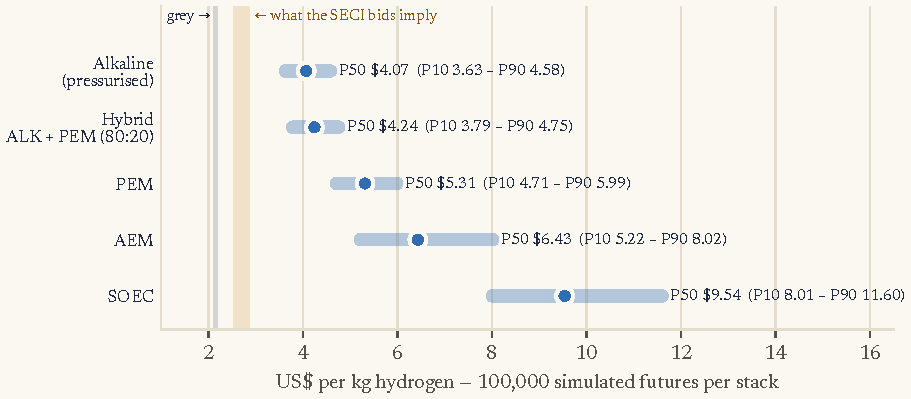
\includegraphics[width=\textwidth]{figures/mc.pdf}
\caption{Monte Carlo results: the bar spans the 10th to 90th percentile, the dot is the median (P50).}\label{fig:mc}
\end{figure}

Two things jump out. First, \textbf{no stack gets below \usd{}3/kg in any meaningful share of futures}; under my ranges the probability is effectively zero for all five. Second, every median sits \emph{above} its base case (alkaline \usd{}4.07 against \usd{}3.83). That is not a bug. Cost overruns are more likely than underruns, so the ranges are skewed to the right, and the ``most likely'' input does not give the ``middle'' outcome. Any project manager who budgets on the most-likely value will overspend more often than not. \confH

\begin{figure}[H]
\centering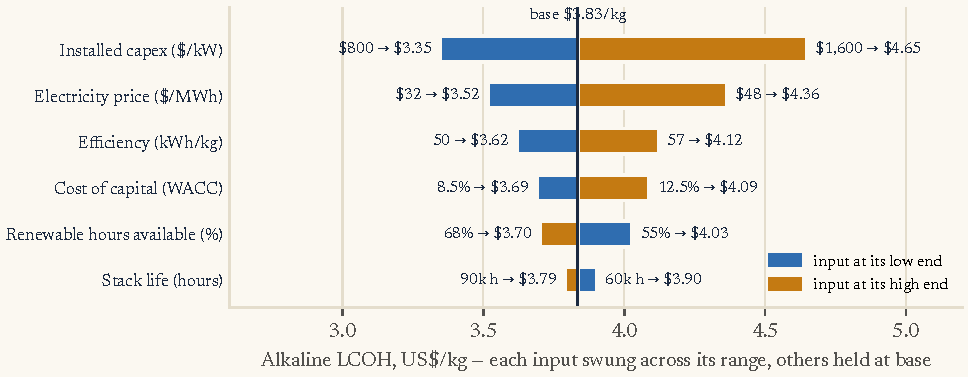
\includegraphics[width=\textwidth]{figures/tornado.pdf}
\caption{Which input moves the alkaline cost most. Each bar swings one input across its full range, holding the rest at base.}
\end{figure}

\begin{finding}[The biggest lever is a project-management lever]
Installed capital cost swings alkaline hydrogen by \usd{}1.30/kg, more than the electricity price (\usd{}0.84) and far more than stack life (\usd{}0.11). In other words, \textbf{the cost of green hydrogen is decided less in the lab than on the construction site}: in the engineering contract, the estimate's maturity and the control of scope creep. That is exactly the territory of our PRM project. \confH
\end{finding}

\subsubsection{What the market is betting.}
India has real prices to test the model against. The thirteen green-ammonia auctions under SIGHT Mode 2A, Tranche I, allocated all 724,000 tonnes a year on 10-year fixed-price contracts \cite{seci2025}.

\begin{figure}[H]
\centering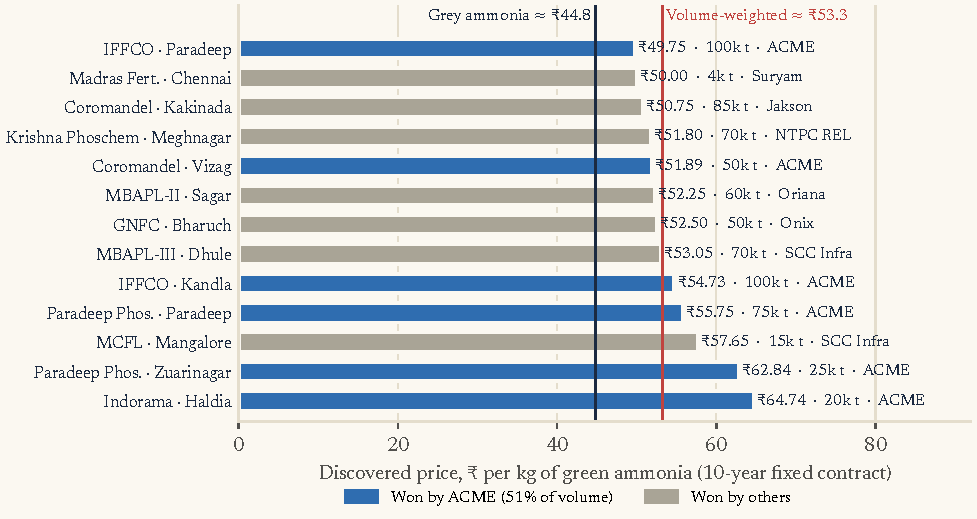
\includegraphics[width=\textwidth]{figures/seci.pdf}
\caption{All 13 SECI green-ammonia auctions (2025), winners and discovered prices. Data: SECI result sheet \cite{seci2025}; grey ammonia benchmark \usd{}515/t \cite{pvm2025} converted at ₹87.}
\end{figure}

The volume-weighted price is \textbf{₹53.27 per kg of ammonia, about \usd{}612 a tonne}, roughly 19\% above grey ammonia's \usd{}515. (JMK Research, using local prices, puts the lowest bid only 10\% above grey \cite{jmkammonia2025}.) ACME alone won 51\% of the volume. Bids were razor-close: at IFFCO Kandla the top three were ₹54.73, ₹54.98 and ₹55.48 \cite{seci2025}. A modest top-up helps: ₹8.82, ₹7.06 and ₹5.30 per kg of ammonia in years one to three \cite{sq2024}. \confH

Strip out a reasonable \usd{}100–160 per tonne for making ammonia from hydrogen (my assumption, \confL), divide by the 0.178 tonnes of hydrogen in each tonne of ammonia, and the bids imply hydrogen at roughly \textbf{\usd{}2.5–2.9/kg}. That is a full dollar below my base case. So I asked the finance question: \emph{what would you have to believe for that price to make money?}

\begin{figure}[H]
\centering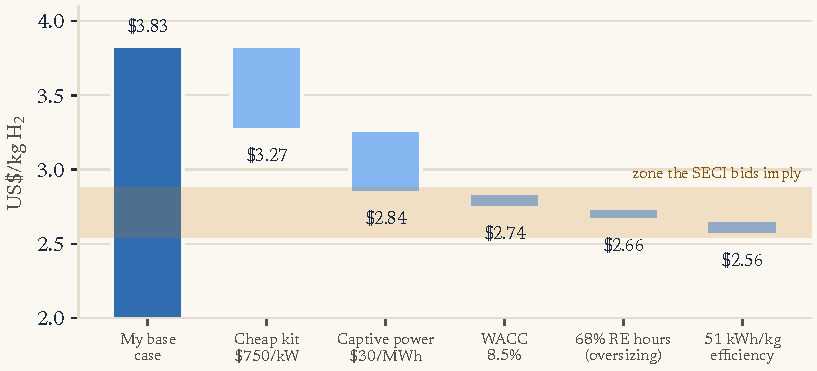
\includegraphics[width=\textwidth]{figures/ladder.pdf}
\caption{``What you have to believe'': stacking favourable assumptions on the alkaline base case until it reaches the price the auctions imply.}
\end{figure}

\begin{finding}[Key finding \textbullet\ the winning bids need almost everything to go right]
To reach the auction-implied cost, a developer needs cheap equipment (about \usd{}750/kW installed), captive power near \usd{}30/MWh, a cost of capital near 8.5\%, heavy oversizing to run 68\% of hours, \emph{and} best-in-class efficiency, all at once. Large groups with their own renewable fleets and balance sheets may get there. For a new entrant it leaves almost no buffer. In auction theory this is the \textbf{winner's curse}: in a tight reverse auction, the winner is often the bidder who was most optimistic, not the one with the lowest true cost. Delivery risk on these contracts deserves close watching. \confM
\end{finding}

The refinery market tells a similar story with longer contracts. Indian Oil's Panipat tender went to L\&T at ₹397/kg (about \usd{}4.6) for 25 years \cite{jmkiocl2025}; Numaligarh Refinery's went to NeuEN Green Energy at ₹279/kg (about \usd{}3.1) in February 2026 \cite{rwnrl2026}. \confH

\subsection{Supply-chain feasibility}\label{sec:supply}

\begin{plainwords}[The iridium arithmetic]
PEM electrolysers need iridium, one of the rarest metals mined. The world produces only about 7–8 tonnes a year, around 95\% of it from South Africa and Zimbabwe, and today's PEM designs use roughly 400 kg per gigawatt \cite{h2tech2022}. Do the division: \textbf{even if every gram of the world's iridium went into PEM, it would cover only about 17–20 GW a year}. At a realistic 20–40\% share, that is roughly 3.5–8 GW a year (my arithmetic). Cutting iridium use by 75\% per gigawatt, which industry believes is achievable, would quadruple that \cite{h2tech2022}. \confM
\end{plainwords}

\begin{table}[H]\centering\tablefont
\caption{Supply-chain exposure by stack. Score: 5 = easy to source, diversified; 1 = fragile.}
\begin{tabularx}{\textwidth}{@{}p{22mm} L L c@{}}
\toprule
\thead{Stack} & \thead{Critical input and where it comes from} & \thead{Indian position} & \thead{Score}\\ \midrule
Alkaline & Nickel, steel, diaphragms; makers concentrated in China (about 60\% of global factory capacity) \cite{argus2026} & Domestic factories under the 3 GW incentive scheme \cite{rw2025} & \score{4}\\
Hybrid & Alkaline inputs plus a small PEM slice & As alkaline, plus a modest import & \score{4}\\
PEM & Iridium and platinum, roughly 95\% from southern Africa \cite{h2tech2022} & Import-dependent for catalysts & \score{2}\\
AEM & Nickel and iron catalysts, no precious metals \cite{irena2020}; supplier base tiny & One licensed factory announced \cite{enki2026} & \score{3}\\
SOEC & Ceramics, perovskites; very few makers & None & \score{2}\\
\bottomrule
\end{tabularx}
\end{table}

Three cross-cutting supply risks apply to every stack. \textbf{Currency}: imported kit is priced in dollars, and the rupee moved from about 86.6 to 91.9 per dollar over 2025 \cite{skfert2026}. \textbf{Long-lead items}: Gemini's brief puts large compressors at 18–24 months and switchgear at 12–16 months \cite{gemini2026}; I could not verify this \confL. \textbf{Water}: desalination adds at most about \usd{}0.10/kg and about 1\% of the electricity \cite{rmi2023}, so a coastal site turns water from a political risk into a small cost. \confH

\subsection{Technical and operational risk}

The core operational problem is simple to state: \textbf{the sun and wind are variable, and the ammonia loop wants a steady diet}. Each stack copes differently.

\begin{table}[H]\centering\tablefont
\caption{Technical and operational risk. Score: 5 = low risk for us; 1 = high risk.}
\begin{tabularx}{\textwidth}{@{}p{22mm} L L c@{}}
\toprule
\thead{Stack} & \thead{Main technical risk} & \thead{How we would manage it} & \thead{Score}\\ \midrule
Alkaline & Slow ramping; a pressurised unit idles below about 40\% load and wastes the morning and evening shoulders of solar \cite{ammoniaenergy2023} & Oversize renewables, add a battery or hydrogen buffer; atmospheric units can turn down to 15\% & \score{4}\\
Hybrid & Two technologies, two OEMs, one control system & One integrator under a single performance guarantee & \score{3}\\
PEM & Shorter stack life; ultra-pure water; iridium cost at stack replacement & Long-term service agreement with degradation guarantees & \score{3}\\
AEM & Durability not yet proven at multi-MW scale in the field \cite{enki2026} & Pilot-scale only until field hours exist & \score{1}\\
SOEC & Under 20,000 h stack life, needs constant high heat \cite{irena2020}; maker pausing production \cite{h2central2026} & Only beside an industrial heat source & \score{1}\\
\bottomrule
\end{tabularx}
\end{table}

Safety applies to all five. Hydrogen leaks easily and embrittles some steels, and ammonia is toxic. Indian plants need approval from the Petroleum and Explosives Safety Organisation (PESO), as the Jind station did, along with leak detection, ventilation and automatic shut-off \cite{skh2train2026}. \confH

\subsection{Value created per rupee spent}

To make ``value per rupee'' concrete I use one plain question: \emph{for every ₹100 we spend making green hydrogen, how many rupees' worth of grey hydrogen, and of the carbon it would have released, do we replace?} If the answer were above ₹100, green hydrogen would pay for itself with no contract or subsidy.

\begin{figure}[H]
\centering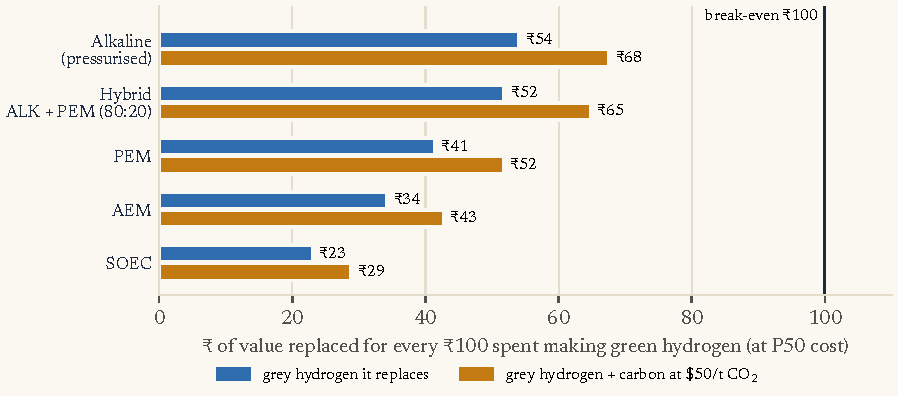
\includegraphics[width=\textwidth]{figures/value.pdf}
\caption{Value replaced per ₹100 spent, at each stack's P50 cost. Grey hydrogen at \usd{}2.2/kg \cite{tribune2025}; 11 kg \coo{} per kg \cite{ieaghr2024}; the \usd{}50/t carbon price is illustrative, not an Indian market price.}
\end{figure}

\begin{table}[H]\centering\tablefont
\caption{What ₹1 crore buys over the plant's life, at P50 cost and ₹90/\usd{}.}
\begin{tabularx}{\textwidth}{@{}L C C C@{}}
\toprule
\thead{Stack} & \thead{Hydrogen per ₹1 crore} & \thead{\coo{} avoided per ₹1 crore} & \thead{Value per ₹100 (with carbon)}\\ \midrule
Alkaline (pressurised) & 27.3 t & 300 t & ₹54 (₹68)\\
Hybrid ALK + PEM & 26.2 t & 288 t & ₹52 (₹65)\\
PEM & 20.9 t & 230 t & ₹41 (₹52)\\
AEM & 17.3 t & 190 t & ₹34 (₹43)\\
SOEC & 11.6 t & 128 t & ₹23 (₹29)\\
\bottomrule
\end{tabularx}
\end{table}

\begin{finding}[Key finding \textbullet\ no stack pays for itself yet, so the contract is the business]
Even the best stack replaces only about ₹54 of grey hydrogen for every ₹100 spent, or ₹68 if carbon is priced at \usd{}50 a tonne. The gap has to be closed by a contract (SECI's fixed price, a refinery's 25-year deal), a subsidy, or a carbon price. This is why I keep saying the offtake contract \emph{is} the business. The technology choice decides how big a gap the contract has to close. \confH
\end{finding}

\subsection{The scorecard}

Figure~\ref{fig:scores} pulls the five criteria together and adds two more: how well a stack fits India's solar-and-wind supply, and its future upside. Every column is turned so that \textbf{5 is good for us}.

\begin{figure}[H]
\centering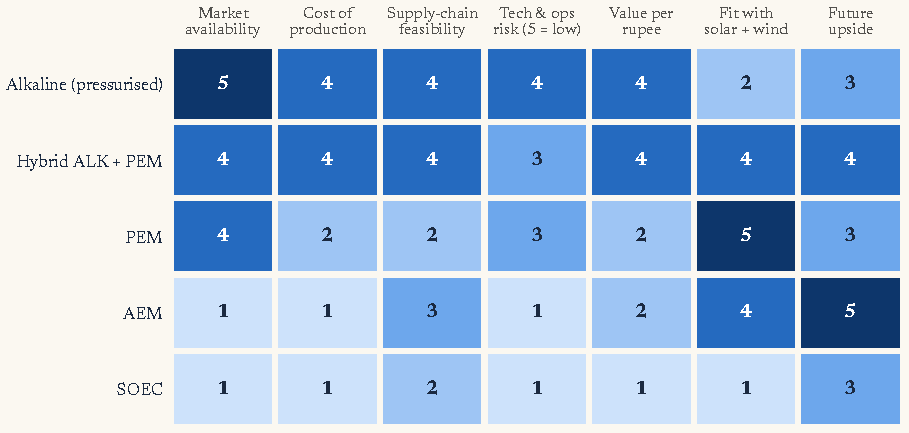
\includegraphics[width=0.96\textwidth]{figures/scores.pdf}
\caption{Technology scorecard (1 = very low, 5 = very high; higher is better in every column). Each score is justified in Sections 3.2–3.7.}\label{fig:scores}
\end{figure}

How you weight the columns depends on who you are. A lender or project manager cares most about cost and risk. A venture investor cares most about upside and owning a scarce position. I scored both.

\begin{table}[H]\centering\tablefont
\caption{Weighted totals under two lenses (out of 5).}
\begin{tabularx}{\textwidth}{@{}L c c L@{}}
\toprule
\thead{Stack} & \thead{Project-finance lens} & \thead{Venture lens} & \thead{Reading}\\ \midrule
Alkaline (pressurised) & \textbf{3.90} & 3.55 & Best for the bankable core\\
Hybrid ALK + PEM & 3.80 & \textbf{3.90} & Best balance; top under the venture lens\\
PEM & 2.85 & 2.80 & Good flexibility, costly and iridium-bound\\
AEM & 1.85 & 3.00 & A real option, not a foundation\\
SOEC & 1.20 & 1.80 & Wrong place, wrong time for us\\ \midrule
\multicolumn{4}{@{}p{\textwidth}@{}}{\footnotesize\itshape Project-finance weights: cost 25\%, risk 20\%, market 15\%, value 15\%, supply 10\%, fit 10\%, upside 5\%. Venture weights: upside 30\%, supply 20\%, cost 15\%, risk 10\%, value 10\%, fit 10\%, market 5\%.}\\
\bottomrule
\end{tabularx}
\end{table}
